\section{Listen}
\subsection{Speicherung mehrerer Elemente desselben Typs}
\begin{itemize}
  \item Array: wenn die Anzahl Elemente statisch ist \\ $\rightarrow$  \lstinline{double statArray[20];} 
  \item Dynamisch allozierter Array: wenn erst zur Laufzeit die Grösse festgelegt wird, dann aber fix bleibt \\ $\rightarrow$ 
  \lstinline{double* dynArray = new double[varSize];}
  \item Liste: wenn die Anzahl Elemente erst zur Laufzeit bekannt ist und laufend ändert
\end{itemize}

\subsection{Eigenschaften einer Liste}
\begin{itemize}
  \item Eine Liste ist eine sequentielle Anordnung von Listenelementen.
  \item Die Listenelemente, auch Knoten (Node) genannt, werden miteinander mittels Pointer verbunden.
  \item Listenanfang: Muss immer gegeben sein, da von diesem ausgegangen wird. 
  \item Listenende: Muss immer gekennzeichnet werden. Wird durch Nullpointer definiert
  \item Besitzt die Grundoperationen: Element einfügen (insert), ELement löschen (delete), Element suchen (search)
\end{itemize}

\subsection{Einfach verkettete Liste - Single Linked List}
\begin{itemize}
  \item Eine einfach verkettete Liste verbindet die Listenelemente nur einfach, d.h. es gibt eine Pointerverbindung nur in eine Richtung.
  \item Rückwärts kann nicht navigiert werden, es geht nur von vorne nach hinten.
  \item Nachteil beim Löschen: da keine Rückwärtsnavigation möglich ist, muss mit einem zusätzlichen Hilfspointer gearbeitet werden.
\end{itemize}

\subsubsection{Definition eines Listenelementes}
\begin{flushleft}
  {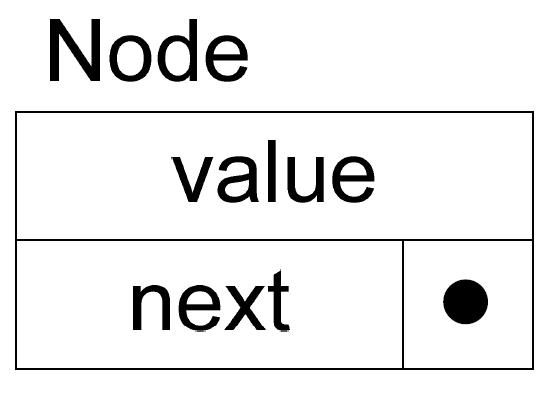
\includegraphics[width=0.1\textwidth]{images/Listen/SLL.png}}
  \label{Fig: Single Linked List}
\end{flushleft}
\lstinputlisting[language=C++]{code/Node_EinfachVerketteteListe.cpp}

\subsubsection{Bezeichnung des Listenanfangs}
\begin{flushleft}
  {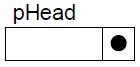
\includegraphics[width=0.1\textwidth]{images/Listen/SLL_Anfang.jpg}}
  \label{Fig: Single Linked List}
\end{flushleft}
\lstinputlisting[language=C++]{code/Listenanfang_EinfachVerketteteListe.cpp}

\subsubsection{Bezeichnung des Listenendes}
\begin{itemize}
  \item Das Listenende wird mit einem Nullpointer gekennzeichnet.
\end{itemize}
\begin{flushleft}
  {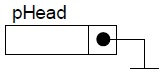
\includegraphics[width=0.15\textwidth]{images/Listen/SLL_Ende.jpg}}
  \label{Fig: Single Linked List}
\end{flushleft}

\subsubsection{Listenelement einfügen}
\begin{flushleft}
{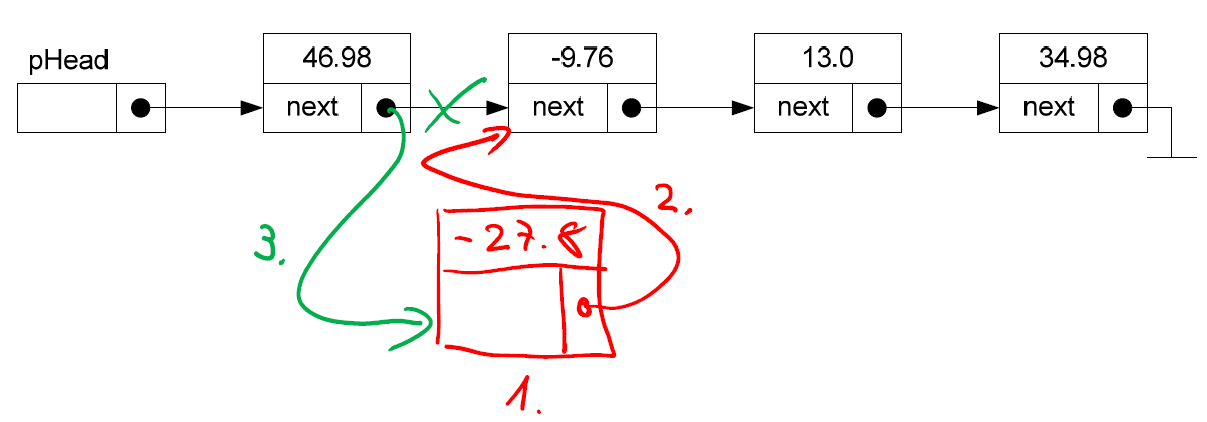
\includegraphics[width=0.5\textwidth]{images/Listen/SLL_Insert.png}}
\label{Fig: Element bei SLL einf"ugen}
\end{flushleft}
\lstinputlisting[language=C++]{code/ListenelementEinfuegen_EinfachVerketteteListe.cpp}

\subsubsection{Listenelement löschen}
\begin{flushleft}
{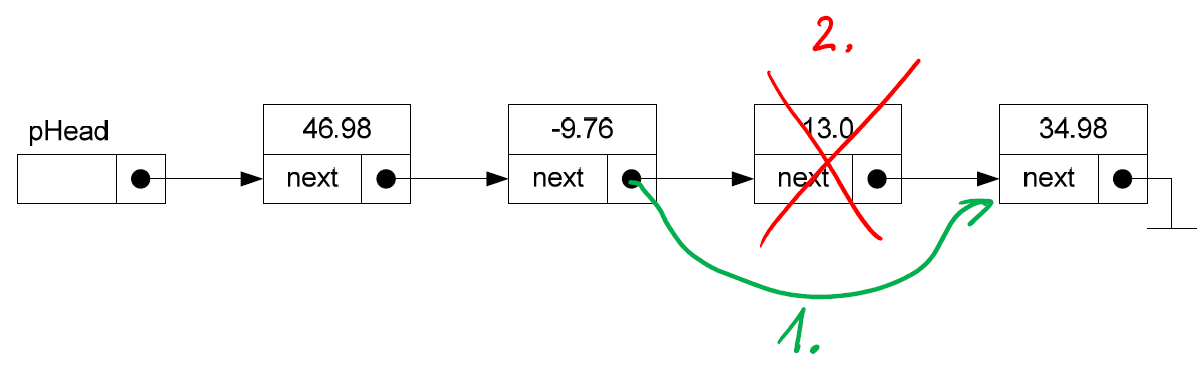
\includegraphics[width=0.5\textwidth]{images/Listen/SLL_Delete.png}}
\label{Fig: Element bei SLL l"oschen}
\end{flushleft}
\lstinputlisting[language=C++]{code/ListenelementLoeschen_EinfachVerketteteListe.cpp}

\subsubsection{Listenelement suchen}
\lstinputlisting[language=C++]{code/ListenelementSuchen_EinfachVerketteteListe.cpp}


\subsection{Doppelt verkettete Liste - Double Linked List}
\begin{itemize}
  \item Eine doppelt verkettete Liste verbindet die Listenelemente in beiden Richtungen.
  \item Dadurch kann einfach in der Liste navigiert werden, speziell rückwärts beim Löschen oder Einfügen.
  \item Der Verdrahtungsaufwand ist grösser als bei der einfach verketteten Liste.
  \item Jeder Knoten braucht einen Pointer mehr, d.h. der Speicherbedarf nimmt leicht zu.
\end{itemize}

\subsubsection{Definition eines Listenelementes}
\begin{flushleft}
  {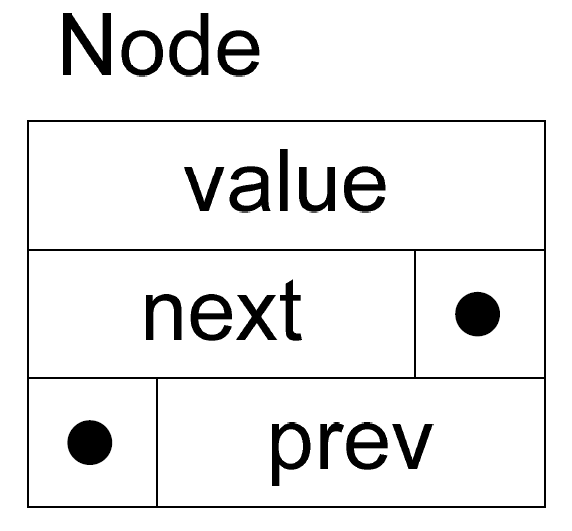
\includegraphics[width=0.1\textwidth]{images/Listen/DLL.png}}
  \label{Fig: Double Linked List}
\end{flushleft}
\lstinputlisting[language=C++]{code/Node_DoppeltVerketteteListe.cpp}

\subsubsection{Bezeichnung des Listenanfangs}
\begin{flushleft}
  {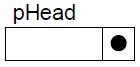
\includegraphics[width=0.1\textwidth]{images/Listen/SLL_Anfang.jpg}}
  \label{Fig: Single Linked List}
\end{flushleft}
\lstinputlisting[language=C++]{code/Listenanfang_EinfachVerketteteListe.cpp}

\subsubsection{Bezeichnung des Listenendes}
\begin{itemize}
  \item Das Listenende wird mit einem Nullpointer gekennzeichnet.
\end{itemize}
\begin{flushleft}
  {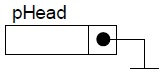
\includegraphics[width=0.15\textwidth]{images/Listen/SLL_Ende.jpg}}
  \label{Fig: Single Linked List}
\end{flushleft}

\subsubsection{Listenelement einfügen}
\begin{flushleft}
{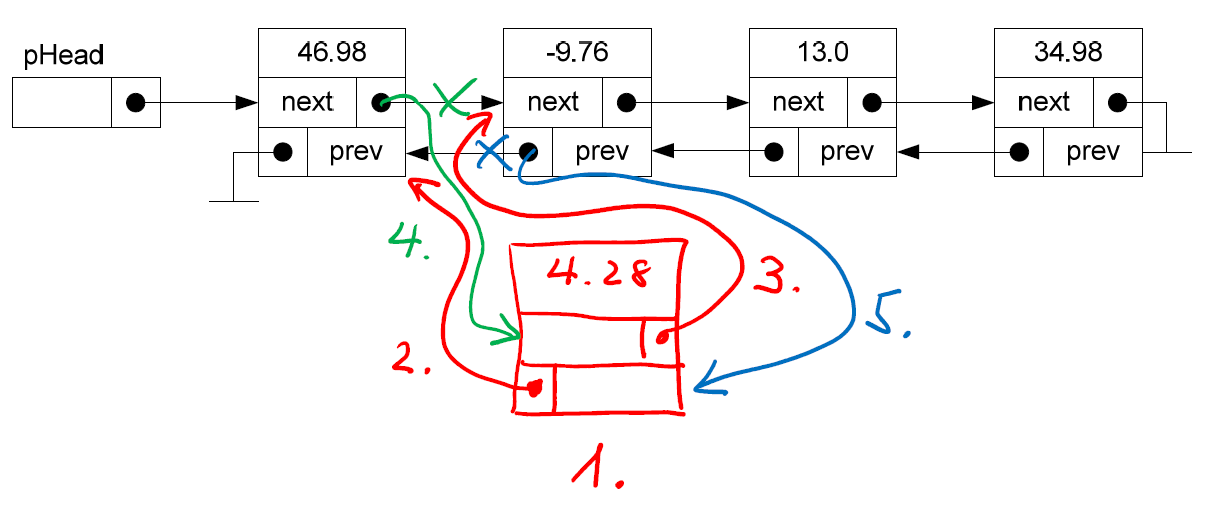
\includegraphics[width=0.5\textwidth]{images/Listen/DLL_Insert.png}}
\label{Fig: Element bei DLL einf"ugen}
\end{flushleft}
\lstinputlisting[language=C++]{code/ListenelementEinfuegen_DoppeltVerketteteListe.cpp}

\subsubsection{Listenelement löschen}
\begin{flushleft}
{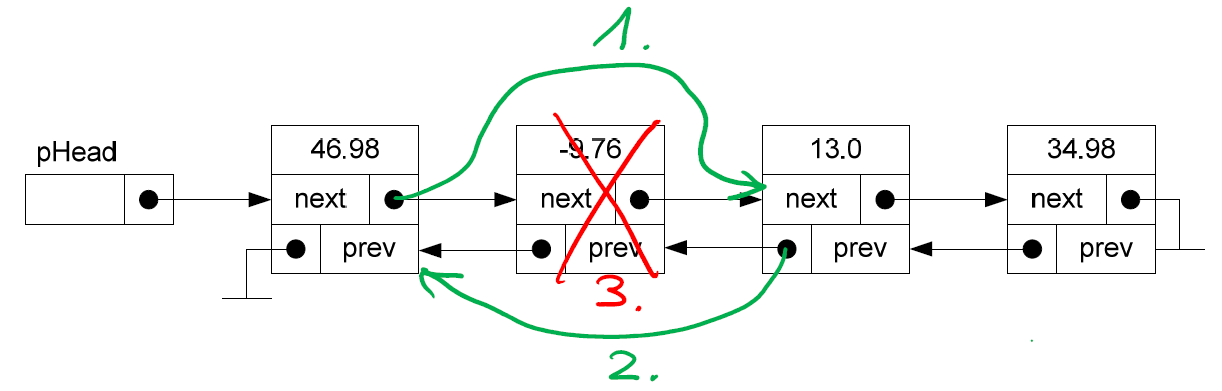
\includegraphics[width=0.5\textwidth]{images/Listen/DLL_Delete.png}}
\label{Fig: Element bei DLL l"oschen}
\end{flushleft}
\lstinputlisting[language=C++]{code/ListenelementLoeschen_DoppeltVerketteteListe.cpp}

\subsubsection{Listenelement suchen}
\lstinputlisting[language=C++]{code/ListenelementSuchen_DoppeltVerketteteListe.cpp}